

Las l\'ineas de emisi\'on de un l\'aser de semiconductor se obtienen del espectro \'optico, definido como el m\'odulo cuadrado de la transformada de Fourier del campo el\'ectrico, que depende de la potencia del l\'aser y de la fase \'optica de \'este. Para un l\'aser en corriente cont\'inua, el campo el\'ectrico, sin ningún tipo de ruido,  alcanza un valor constante y as\'i, su transformada de Fourier es una funci\'on delta de Dirac $\delta(\nu-\nu_0)$, obteniendo en el espectro una \'unica l\'inea de emisi\'on bien definida para una cierta frecuencia $\nu_0$.

	\begin{figure}[H]
		\centering
		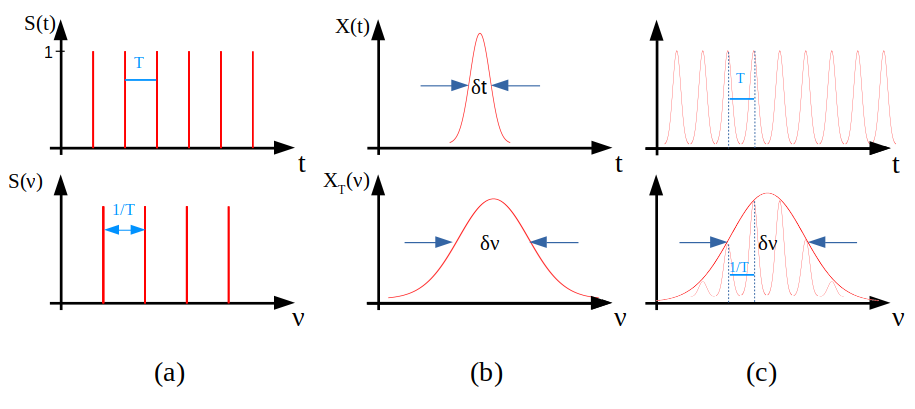
\includegraphics[width=1.0\linewidth]{OFC.png}
		\caption{\label{Img:FFtPulsos}Esquemas de la relaci\'on entre la funci\'on de la evolución temporal de una señal (fila superior) y su transformada de Foutier en el espacio de frecuencias $\nu$ (fila inferior), para tres tipos de señales: (a) tren de pulsos infinitamente estrechos, (b) un \'unico pulso con anchura (FWHM) $\delta t$ y (c) un tren de pulsos con anchura (FWHM) $\delta t$.}
	\end{figure}

Si se tiene una señal formada por un tren de pulsos infinitamente estrechos separados un tiempo $T$, se sabe por su transformada de Fourier que el espectro \'optico en frecuencias ha de ser otro tren de pulsos infinitamente estrechos, pero separados $1/T$ (Figura \ref{Img:FFtPulsos} (a)). Sin embargo, en los experimentos no es posible obtener pulsos infinitamente estrechos sino que se tiene pulsos con una cierta anchura FWHM (siglas en ingl\'es de anchura a media altura). Su espectro \'optico ser\'a otro pulso con FWHM $\delta\nu$ (Figura \ref{Img:FFtPulsos} (b)), donde se tiene que se ha de cumplir que el producto $\delta\nu\delta t$ es contante. En la ecuaci\'on \ref{eq:types} se muestran diferentes valores del producto $\delta\nu\delta t$ seg\'un la forma del pulso en $t$.

	\begin{equation}
		\delta\nu\delta t = 
			\left\{\begin{matrix}
				& 0.315 & \textrm{sech}^2 \\
				& 0.44 & \textrm{Gaussiana}
			\end{matrix}\right.
		\label{eq:types}
	\end{equation}

	Un tren de pulsos con ancho $\delta t$ ser\'a la combinaci\'on de las dos señales anteriores y su expresi\'on vendr\'a dada por la convoluci\'on de ambas funciones. Su transformada de Fourier es el producto de las transformadas de Fourier de las funciones anteriores, obteniendo un espectro formado por pulsos estrechos con una separaci\'on entre ellos de $1/T$ y cuya envolvente viene dada por la forma del espectro del pulso individual (Figura \ref{Img:FFtPulsos} (c)). A este tipo de espectros se les denomina peines.

Los peines de frecuencia \'optica (OFC por sus siglas en ingl\'es) son fuentes \'opticas formados por un gran n\'umero l\'ineas de emisi\'on con un espaciado preciso y equidistante. Los OFC vienen caracterizados tanto por la forma de la envolvente como por la separaci\'on entre los picos, obteniendo OFC de mayor calidad para envolventes anchas y regulares. Esto se obtiene para campos el\'ectricos con pulsos regulares, estrechos e intensos.

Cabe recordar que los espectros \'opticos se obtienen a partir del campo el\'ectrico, cuyo comportamiento puede ser descrito mediante una ecuaci\'on de ondas de la que obtenemos una fase \'optica $\Phi$ y una amplitud relacionada con la potencia del l\'aser. Mientras que para la potencia puede ser descrita con el desarrollo anterior, los efectos de la fase \'optica son diferentes. De esta forma, los efectos que se observan al estudiar los OFC son el resultado de la evolución de amplitud y fase óptica. Uno de los efectos de la fase \'optica en los OFC se puede observar en la anchura de las l\'ineas espectrales, que disminuye para fases menos aleatorias.

Pese a que existen diferentes mecanismos de creaci\'on de OFC, en este trabajo se estudiar\'an solo los m\'etodos de generaci\'on de OFC mediante \gs\ y por inyecci\'on \'optica.

	\subsection{Encendido por Ganancia}
		\label{Intr:OFC:GS}

		El \gs\ (\textit{Gain-Switching} en ingl\'es) es una t\'ecnica mediante la cu\'al se alcanza r\'apidamente un alto valor para la ganancia del l\'aser \cite{principles}. Esta t\'ecnica permite generar pulsos del l\'aser de corta duraci\'on y grandes picos de potencia, pudiendo obtener OFC de gran calidad. El \gs\ consiste en conseguir que la inversi\'on de poblaci\'on, y por tanto la ganancia, alcance un valor muy por encima del valor umbral antes de que la densidad de fotones tenga tiempo de alcanzar un nivel suficiente para reducir la inversi\'on. 
		
		El uso de pulsos de bombeo suficientemente r\'apidos, corriente eléctrica en el caso de láseres de semiconductor, permite alcanzar la condici\'on de la inversi\'on de poblaci\'on, alcanzando el \gs. Mediante el uso de corriente de inyecci\'on modulada por una funci\'on sinusoidal se puede controlar la forma del pulso de bombeo a partir de la amplitud y frecuencia, controlando los valores \'optimos de ancho y potencia de pulsos ópticos para el \gs.

	\subsection{Inyección Óptica}

		Otro m\'etodo de generaci\'on de OFC es mediante la inyecci\'on \'optica. \'Esta consiste en inyectar fotones provenientes de un segundo l\'aser al l\'aser de semiconductor. Bajo determinadas condiciones de potencia y frecuencia del láser que inyecta, se pueden obtener OFC. Puesto que se va a trabajar con l\'aseres de semiconductor, cabe destacar la gran sensibilidad de \'estos a la inyecci\'on \'optica debida entre otras cosas al acoplamiento amplitud-fase a trav\'es del factor de ensanchamiento del ancho de l\'inea \cite{tfgPopp}.

		Para un l\'aser sin inyecci\'on de luz, la fase evoluciona de manera aleatoria en el tiempo, principalmente debido a la emisión espontánea, y as\'i se obtienen anchos de l\'inea grandes (del orden del MHz para un láser monomodo). Sin embargo, al realizarse la inyecci\'on de luz las caracter\'isticas de la fase del l\'aser inyectado pasan a estar determinadas por la inyecci\'on , pudiendo obtener un fase menos aleatoria si el espectro óptico del láser que inyecta es más estrecho. De esta forma se tiene un menor ruido en la fase, obteniendo picos m\'as estrechos en el OFC.

		Este m\'etodo tambi\'en puede producir otro fen\'omeno bajo unas condiciones determinadas, conocido como bloqueo por inyecci\'on. Si se tiene una inyecci\'on \'optica de fotones de frecuencia diferente a la del l\'aser inyectado, bajo ciertas condiciones se puede dar que el l\'aser inyectado comience a emitir en la frecuencia del l\'aser que inyecta, desapareciendo la emisi\'on del l\'aser inyectado a la frecuencia de emisión en solitario.

	\subsection{Aplicaciones}

		Tal y como se ha descrito anteriormente, los OFC presentan l\'ineas de emisi\'on bien definidas, perfectamente equiespaciadas y con una fuerte correlaci\'on en la fase \cite{desi2017development}. \'Esto les convierte en una herramienta de gran inter\'es para la espectroscop\'ia y las cominucaciones \'opticas.

		Los OFC permiten obtener varias l\'ineas de emisi\'on bien definidas y equiespaciadas para diferentes longitudes de onda a partir de la emisi\'on de un \'unico l\'aser. De esta forma permite sustituir sistemas formados por multiples l\'aseres independientes, disminuyendo costes, consumo de potencia y complejidad. Estos sistemas con láseres independientes se utilizan en la actualidad en comunicaciones ópticas de alta velocidad y se les llama DWDM (\textit{Dense wavelength division multiplexing} en inglés). Si a esto se le añade la capacidad de ajustar la frecuencia de separación entre las líneas o la longitud de onda de éstas, se obtiene unas cualidades de gran importancia para su uso en comunicaciones \'opticas. Esta capacidad de ajuste se puede obtener con los OFC en láseres de semiconductor en \gs. Además, la correlación de fases del OFC presenta multiples ventajas para la transmisión por fibra óptica, pudiendo ser utilizada para cancelar los efectos no lineales que distorsionan la información que viaja por la fibra, pudiendo recuperar dicha información \cite{temprana2015overcoming}. Para las aplicaciones en comunicaciones ópticas de alta velocidad, son deseables OFC con una gran separación entre líneas. Sin embargo, para las aplicaciones de espectroscopía óptica se requieren OFC con separación entre líneas pequeña, para obtener espectros con buena resolución.
